\documentclass{sig-alternate}
\usepackage{hyperref}	% make links (like references, links to Sections, ...) clickable
\usepackage{enumitem}	% tighten itemize etc by appending '[noitemsep,nolistsep]'
\usepackage{cleveref}

\graphicspath{{img/}} % put the images in this folder

\begin{document}

% Copyright
\setcopyright{waclicense}


%% DOI
%\doi{10.475/123_4}
%
%% ISBN
%\isbn{123-4567-24-567/08/06}
%
%%Conference
%\conferenceinfo{PLDI '13}{June 16--19, 2013, Seattle, WA, USA}
%
%\acmPrice{\$15.00}

%
% --- Author Metadata here ---
\conferenceinfo{Web Audio Conference WAC-2016,}{April 4--6, 2016, Atlanta, USA}
\CopyrightYear{2016} % Allows default copyright year (20XX) to be over-ridden - IF NEED BE.
%\crdata{0-12345-67-8/90/01}  % Allows default copyright data (0-89791-88-6/97/05) to be over-ridden - IF NEED BE.
% --- End of Author Metadata ---

\title{Web Audio Evaluation Tool: A framework for subjective assessment of audio}
%\subtitle{[Extended Abstract]
%\titlenote{A full version of this paper is available as
%\textit{Author's Guide to Preparing ACM SIG Proceedings Using
%\LaTeX$2_\epsilon$\ and BibTeX} at
%\texttt{www.acm.org/eaddress.htm}}}
%
% You need the command \numberofauthors to handle the 'placement
% and alignment' of the authors beneath the title.
%
% For aesthetic reasons, we recommend 'three authors at a time'
% i.e. three 'name/affiliation blocks' be placed beneath the title.
%
% NOTE: You are NOT restricted in how many 'rows' of
% "name/affiliations" may appear. We just ask that you restrict
% the number of 'columns' to three.
%
% Because of the available 'opening page real-estate'
% we ask you to refrain from putting more than six authors
% (two rows with three columns) beneath the article title.
% More than six makes the first-page appear very cluttered indeed.
%
% Use the \alignauthor commands to handle the names
% and affiliations for an 'aesthetic maximum' of six authors.
% Add names, affiliations, addresses for
% the seventh etc. author(s) as the argument for the
% \additionalauthors command.
% These 'additional authors' will be output/set for you
% without further effort on your part as the last section in
% the body of your article BEFORE References or any Appendices.

% FIVE authors instead of four, to leave space between first two authors.
\numberofauthors{5} %  in this sample file, there are a *total*
% of EIGHT authors. SIX appear on the 'first-page' (for formatting
% reasons) and the remaining two appear in the \additionalauthors section.
%
\author{
% You can go ahead and credit any number of authors here,
% e.g. one 'row of three' or two rows (consisting of one row of three
% and a second row of one, two or three).
%
% The command \alignauthor (no curly braces needed) should
% precede each author name, affiliation/snail-mail address and
% e-mail address. Additionally, tag each line of
% affiliation/address with \affaddr, and tag the
% e-mail address with \email.
%
% 1st. author
\alignauthor Nicholas Jillings\\
       \email{n.g.r.jillings@se14.qmul.ac.uk}
 % dummy author for nicer spacing
 \alignauthor 
% 2nd. author
\alignauthor Brecht De Man\\
       \email{b.deman@qmul.ac.uk}
\and  % use '\and' if you need 'another row' of author names
% 3rd. author
\alignauthor David Moffat\\
       \email{d.j.moffat@qmul.ac.uk}
% 4th. author
\alignauthor Joshua D. Reiss\\
\email{joshua.reiss@qmul.ac.uk}
\and % new line for address
       \affaddr{Centre for Digital Music}\\
       \affaddr{School of Electronic Engineering and Computer Science}\\
       \affaddr{Queen Mary University of London}\\
       \affaddr{Mile End Road,}
       \affaddr{London E1 4NS}\\
       \affaddr{United Kingdom}\\
}
%Centre for Digital Music, School of Electronic Engineering and Computer Science, Queen Mary University of London
%% 5th. author
%\alignauthor Sean Fogarty\\
%       \affaddr{NASA Ames Research Center}\\
%       \affaddr{Moffett Field}\\
%       \email{fogartys@amesres.org}
%% 6th. author
%\alignauthor Charles Palmer\\
%       \affaddr{Palmer Research Laboratories}\\
%       \affaddr{8600 Datapoint Drive}\\
%       \email{cpalmer@prl.com}
%}
% There's nothing stopping you putting the seventh, eighth, etc.
% author on the opening page (as the 'third row') but we ask,
% for aesthetic reasons that you place these 'additional authors'
% in the \additional authors block, viz.
%\additionalauthors{Additional authors: John Smith (The Th{\o}rv{\"a}ld Group,
%email: {\texttt{jsmith@affiliation.org}}) and Julius P.~Kumquat
%(The Kumquat Consortium, email: {\texttt{jpkumquat@consortium.net}}).}
\date{1 October 2015}
% Just remember to make sure that the TOTAL number of authors
% is the number that will appear on the first page PLUS the
% number that will appear in the \additionalauthors section.

\maketitle
\begin{abstract}
Here comes the abstract. 
\end{abstract}


\section{Introduction}

	% Listening tests/perceptual audio evaluation: what are they, why are they important
	% As opposed to limited scope of WAC15 paper: also musical features, realism of sound effects / sound synthesis, performance of source separation and other algorithms... 
	Perceptual evaluation of audio, in the form of listening tests, is a powerful way to assess anything from audio codec quality over realism of sound synthesis to the performance of source separation, automated music production and other auditory evaluations.
	In less technical areas, the framework of a listening test can be used to measure emotional response to music or test cognitive abilities. 
	% maybe some references? If there's space.

	% check out http://link.springer.com/article/10.1007/s10055-015-0270-8 - only paper that cited WAC15 paper

	% Why difficult? Challenges? What constitutes a good interface?
	% Technical, interfaces, user friendliness, reliability 
	Several applications for performing perceptual listening tests currently exist, as can be seen in Table \ref{tab:toolboxes}. The Web Audio Evaluation Toolbox stands out as it does not require proprietary software or a specific platform and provides a wide range of interface and test types in one user friendly environment. Furthermore, it does not require any progamming experience as any test based on the default test types can be configured in the browser as well. Note that the design of an effective listening test further poses many challenges unrelated to interface design, which are beyond the scope of this paper \cite{bech}. 

	% Why in the browser? 
	Web Audio API has important features for performing perceptual tests including sample level manipulation of audio streams \cite{schoeffler2015mushra}, synchronous playback and flexible playback. Being in the browser also allows leveraging the flexible object oriented JavaScript format and native support for web documents, such as the extensible markup language (XML) which is used for configuration and test result files. Using the web also reduces deployment requirements to a basic web server with advanced functionality such as test collection and automatic processing using PHP. As recruiting participants can be very time-consuming, and as for some tests a large number of participants is needed, browser-based tests \cite{schoeffler2015mushra}. However, to our knowledge, no tool currently exists that allows the creation of a remotely accessible listening test. 

	Both BeaqleJS \cite{beaqlejs} and mushraJS\footnote{https://github.com/akaroice/mushraJS} also operate in the browser, however BeaqleJS does not make use of the Web Audio API and therefore lacks arbitrary manipulation of audio stream samples, and neither offer an adequately wide choice of test designs for them to be useful to many researchers. %requires programming knowledge?... 
	
	% only browser-based? 
	\begin{table*}[ht]
    \caption{Table with existing listening test platforms and their features}
    \begin{center}
    	\begin{tabular}{|*{6}{l|}}
    		\hline
    		\textbf{Name} 	& \textbf{Ref.} 	& \textbf{Language} 	& \textbf{Interfaces} 			& \textbf{Remote} 			& \textbf{All UI} 	\\
    		\hline
    		APE 			& \cite{ape}		& MATLAB				& multi-stimulus, 1 axis per attribute 	& 					& 			 \\
    		BeaqleJS		& \cite{beaqlejs}	& JavaScript			& ABX, MUSHRA 					& (not natively supported) 	& 			 \\
    		HULTI-GEN 		& \cite{hultigen}	& MAX 					& See Table \ref{tab:toolbox_interfaces}& 							& \checkmark \\
    		mushraJS		& 					& JavaScript 			& MUSHRA 						& \checkmark				& 	 \\
    		MUSHRAM			& \cite{mushram}	& MATLAB				& MUSHRA						& 							& 			 \\
    		Scale 			& \cite{scale}		& MATLAB				& See Table \ref{tab:toolbox_interfaces} &							&			 \\
    		WhisPER			& \cite{whisper}	& MATLAB				& See Table \ref{tab:toolbox_interfaces}								&							& \checkmark \\
    		\textbf{WAET}	& \cite{waet}		& JavaScript			& \textbf{All of the above}				& \checkmark				& \checkmark \\
    		\hline
    	\end{tabular}
    \end{center}
    \label{tab:toolboxes}
    \end{table*}%

    \begin{table*}[ht]
    \caption{Table with interfaces and which toolboxes support them}
    \begin{center}
    	\begin{tabular}{|*{5}{l|}}
    		\hline
    		\textbf{Interface} 									& \textbf{HULTI-GEN} 	& \textbf{Scale} 	& \textbf{WhisPER} 	& \textbf{WAET} \\
    		\hline
    		MUSHRA (ITU-R BS. 1534)								& \checkmark 			&					&					& \checkmark 	\\
    		Rank scale 											& \checkmark 			&					&					& \checkmark	\\
			Likert scale										& \checkmark 			&					& \checkmark		& \checkmark	\\
			ABC/HR (ITU-R BS. 1116)								& \checkmark 			&					&					& \checkmark	\\
			-50 to 50 Bipolar with Ref							& \checkmark 			&					& 					& \checkmark	\\
			Absolute Category Rating (ACR) Scale				& \checkmark 			&					&					& \checkmark	\\
			Degredation Category Rating (DCR) Scale				& \checkmark 			&					&					& \checkmark	\\
			Comparison Category Rating (CCR) Scale				& \checkmark 			&					& \checkmark		& \checkmark	\\
			9 Point Hedonic Category Rating Scale				& \checkmark 			&					& \checkmark		& \checkmark	\\
			ITU-R 5 Point Continuous Impairment Scale			& \checkmark 			&					&					& \checkmark	\\
			Pairwise Comparison / AB test						& \checkmark 			&					&					& \checkmark	\\
			Multi-attribute ratings								& \checkmark 			&					&					& \checkmark	\\
			ABX Test											& \checkmark 			&					&					& \checkmark	\\
			Adaptive psychophysical methods						& 						&					& \checkmark		&				\\
			Repertory Grid Technique (RGT)						&						&					& \checkmark		&				\\
			Semantic differential								&						& \checkmark		& \checkmark		&				\\
			n-Alternative Forced choice 						&						& \checkmark		&					&				\\

    		\hline
    	\end{tabular}
    \end{center}
    \label{tab:toolbox_interfaces}
    \end{table*}%

        % 
        %Selling points: remote tests, visualisaton, create your own test in the browser, many interfaces, few/no dependencies, flexibility

        To meet the need for a cross-platform, versatile and easy-to-use listening test tool, we previously developed the Web Audio Evaluation Tool \cite{waet} which at the time of its inception was capable of running a listening test in the browser from an XML configuration file, and storing an XML file as well, with one particular interface. We have now expanded this into a tool with which a wide range of listening test types can easily be constructed and set up remotely, without any need for manually altering code or configuration files, and which allows visualisation of the collected results in the browser. In this paper, we discuss these different aspects and explore which future improvements would be possible. Specifically, in Section \ref{sec:architecture} we cover the general implementation aspects, with a focus on the Web Audio API, followed by a discussion of the requirements for successful remote tests in Section \ref{sec:remote}. Section \ref{sec:interfaces} describes the various interfaces the tool supports, as well as how to keep this manageable. Finally, in Section \ref{sec:analysis} we provide an overview of the analysis capabilities in the browser, before summarising our findings and listing future research directions in Section \ref{sec:conclusion}. 

\begin{comment}
        % MEETING 8 OCTOBER
        \subsection{Meeting 8 October}
        \begin{itemize}
        	\item Do we manipulate audio?\\
	        	\begin{itemize}
	        		\item Add loudness equalisation? (test\_create.html) Tag with gains. 
	        		\item Add volume slider? 
	        		\item Cross-fade (in interface node): default 0, number of seconds
	        		\item Also: we use the playback buffer to present metrics of which portion is listened to
	        	\end{itemize}
	        \item Logging system information: whichever are possible (justify others)
	        \item Input streams as audioelements
	       	\item Capture microphone to estimate loudness (especially Macbook)
	       	\item Test page (in-built oscillators): left-right calibration, ramp up test tone until you hear it; optional compensating EQ (future work implementing own filters) --> Highlight issues! 
	       	\item Record IP address (PHP function, grab and append to XML file)
	       	\item Expand anchor/reference options
	       	\item AB / ABX
        \end{itemize}

        \subsubsection{Issues}
        \begin{itemize}
        	\item Filters not consistent (Nick to test across browsers)
        	\item Playback audiobuffers need to be destroyed and rebuilt each time
        	\item Can't get channel data, hardware input/output... 
        \end{itemize}
\end{comment}
	
\section{Architecture}  % title? 'back end'? % NICK
	\label{sec:architecture}

    While WAET uses a sparse subset of the Web Audio API functionality, its performance comes directly from using the Web Audio API for audio playback. Listening tests can convey large amounts of information other than obtaining the perceptual relationship between the audio fragments. Specifically, with WAET one can obtain which parts of the audio fragments were listened to and when, at what point in the audio stream the participant switched to a different fragment, and how a fragment's rating was adjusted over time within a session, to name a few. Not only does this allow to evaluate a wealth of perceptual aspects, but it helps detect poor participants whose results are potentially not representative. 
    
    One of the key initial design parameters for WAET is to make the tool as open as possible to non-programmers and to this end the tool has been designed in such a way that all of the user modifiable options are included in a single XML document. This document is loaded up automatically by the web page and the JavaScript code parses and loads any extra resources required to create the test.
    
    The specification document also contains the URL of the audio fragments for each test page. These fragments are downloaded asynchronously and decoded offline by the Web Audio offline decoder. The resulting buffers are assigned to a custom Audio Objects node which tracks the fragment buffer, the playback bufferSourceNode, the XML information including its unique test ID, the interface object(s) associated with the fragment and any metric or data collection objects. The Audio Object is controlled by an over-arching custom Audio Context node (not to be confused with the Web Audio Context), this parent JS Node allows for session wide control of the Audio Objects including starting and stopping playback of specific nodes.
    
    The only issue with this model is the bufferNode in the Web Audio API, which is implemented as a `use once' object which, once the buffer has been played, the buffer must be discarded as it cannot be instructed to play the buffer again. Therefore on each start request the buffer object must be created and then linked with the stored bufferSourceNode. This is an odd behaviour for such a simple object which has no alternative except to use the HTML5 audio element, however they do not have the ability to synchronously start on a given time and therefore not suited.
    
    The media files supported depend on the browser level support for the initial decoding of information and is the same as the browser support for the HTML5 audio element. Therefore the most widely supported media file is the wave (.WAV) format which can be accpeted by every browser supporting the Web Audio API. The next best supported audio only formats are MP3 and AAC (in MP4) which are supported by all major browsers, Firefox relies on OS decoders and therefore its support is predicated by the OS support.
    
    All the collected session data is returned in an XML document structured similarly to the configuration document, where test pages contain the audio elements with their trace collection, results, comments and any other interface-specific data points.
    
	%A slightly technical overview of the system. Talk about XML, JavaScript, Web Audio API, HTML5. 
	%Describe and/or visualise audioholder-audioelement-... structure. 

	% see also SMC12 - less detail here

	%Which type of files? % WAV, anything else? Perhaps not exhaustive list, but say something along the lines of 'whatever browser supports'
	
	%Streaming audio? % probably not, unless it's easy

	%Compatibility? % not IE, everything else fine? 


	
	
\section{Remote tests} % with previous? 
	\label{sec:remote}

	If the experimenter is willing to trade some degree of control for a higher number of participants, the test can be hosted on a web server so that subjects can take part remotely. This way, a link can be shared widely in the hope of attracting a large amount of subjects, while listening conditions and subject reliability may be less ideal. However, a sound system calibration page and a wide range of metrics logged during the test mitigate these problems. Note also that in some experiments, it may be preferred that the subject has a `real life', familiar listening set-up, for instance when perceived quality differences on everyday sound systems are investigated. 
	Furthermore, a fully browser-based test, where the collection of the results is automatic, is more efficient and technically reliable even when the test still takes place under lab conditions.

	The following features allow easy and effective remote testing: 
	\begin{description}[noitemsep,nolistsep]
		\item[PHP script to collect result XML files] and store on central server. 
		\item[Randomly pick a specified number of pages] to ensure an equal and randomised spread of the different pages (`audioHolders') across participants. 
		\item[Calibration of the sound system (and participant)] by a perceptual pre-test to gather information about the frequency response and speaker configuration - this can be supplemented with a survey.
		% In theory calibration could be applied anywhere??
		% \item Functionality to participate multiple times
		% 	\begin{itemize}[noitemsep,nolistsep]
		% 		\item Possible to log in with unique ID (no password)
		% 		\item Pick `new user' (generates new, unique ID) or `already participated' (need already available ID)
		% 		\item Store XML on server with IDs plus which audioholders have already been listened to
		% 		\item Don't show `post-test' survey after first time
		% 		\item Pick `new' audioholders if available
		% 		\item Copy survey information first time to new XMLs
		% 	\end{itemize}
		\item[Intermediate saves] for tests which were interrupted or unfinished.
		\item[Collect IP address information] for geographic location, through PHP function which grabs address and appends to XML file. 
		\item[Collect Browser and Display information] to the extent it is available and reliable. 
	\end{description}

	
\section{Interfaces} % title? 'Front end'? % Dave
\label{sec:interfaces}

The purpose of this listening test framework is to allow any user the maximum flexibility to design a listening test for their exact application with minimum effort. To this end, a large range of standard listening test interfaces have been implemented. A review of existing listening test frameworks was undertaken and presented in~\Cref{tab:toolboxes}. HULTI-GEN~\cite{hultigen} is a single toolbox that presents the user with a large number of different test interfaces and allows for customisation of each test interface.

To provide users with a flexible system, a large range of `standard' listening test interfaces have been implemented, including: % pretty much the same wording as two sentences earlier
	\begin{itemize}[noitemsep,nolistsep]
		\item MUSHRA (ITU-R BS. 1534)~\cite{recommendation20031534}
		\begin{itemize}
			\item Multiple stimuli are presented and rated on a continuous scale, which includes a reference, hidden reference and hidden anchors.
		\end{itemize}
		\item Rank Scale~\cite{pascoe1983evaluation}
		\begin{itemize}
			\item Stimuli ranked on single horizontal scale, where they are ordered in preference order.
		\end{itemize}
		\item Likert scale~\cite{likert1932technique}
		\begin{itemize}
			\item Each stimuli has a five point scale with values: Strongly Agree, Agree, Neutral, Disagree and Strongly Disagree.
		\end{itemize}
		\item ABC/HR (ITU-R BS. 1116)~\cite{recommendation19971116} (Mean Opinion Score: MOS)
		\begin{itemize}
			\item Each stimulus has a continuous scale (5-1), labeled as Imperceptible, Perceptible but not annoying, slightly annoying, annoying, very annoying.
		\end{itemize}
		\item -50 to 50 Bipolar with Ref
		\begin{itemize}
			\item Each stimulus has a continuous scale -50 to 50 with default values as 0 in middle and a comparison. There is also a provided reference		\end{itemize}
		\item Absolute Category Rating (ACR) Scale~\cite{rec1996p}
		\begin{itemize}
			\item Each stimuli has a five point scale with values: Bad, Poor, Fair, Good, Excellent
		\end{itemize}
		\item Degredation Category Rating (DCR) Scale~\cite{rec1996p}
		\begin{itemize}
			\item Each stimuli has a five point scale with values: (5) Inaudible, (4) Audible but not annoying, (3) slightly annoying, (2) annoying, (1) very annoying.
		\end{itemize}
		\item Comparison Category Rating (CCR) Scale~\cite{rec1996p}
		\begin{itemize}
			\item Each stimuli has a seven point scale with values: Much Better, Better, Slightly Better, About the same, slightly worse, worse, much worse. There is also a provided reference.
		\end{itemize}
		\item 9 Point Hedonic Category Rating Scale~\cite{peryam1952advanced}
		\begin{itemize}
			\item Each stimuli has a seven point scale with values: Like Extremely, Like Very Much, Like Moderate, Like Slightly, Neither Like nor Dislike, dislike Extremely, dislike Very Much, dislike Moderate, dislike Slightly. There is also a provided reference.
			\end{itemize}
		\item ITU-R 5 Point Continuous Impairment Scale~\cite{rec1997bs}
		\begin{itemize}
			\item Each stimuli has a five point scale with values: (5) Imperceptible, (4) Perceptible but not annoying, (3) slightly annoying, (2) annoying, (1) very annoying. There is also a provided reference.
		\end{itemize}
		\item Pairwise Comparison (Better/Worse)~\cite{david1963method}
		\begin{itemize}
			\item A reference is provided and ever stimulus is rated as being either better or worse than the reference.
		\end{itemize}
		\item APE style \cite{ape}
		\begin{itemize}
			\item Multiple stimuli on a single horizontal slider for inter-sample rating.
		\end{itemize}
		\item Multi attribute ratings
		\begin{itemize}
			\item Multiple stimuli as points on a 2D plane for inter-sample rating (eg. Valence Arousal)
		\end{itemize}
		\item AB Test~\cite{lipshitz1981great}
		\begin{itemize}
			\item Two stimuli are presented at a time and the participant has to select a preferred stimulus.
		\end{itemize}
		\item ABX Test~\cite{clark1982high}
		\begin{itemize}
			\item Two stimuli are presented along with a reference and the participant has to select a preferred stimulus, often the closest to the reference.
		\end{itemize}
	\end{itemize}
	
	While implementing all of these interfaces, it is possible to include any number of references, anchors, hidden references and hidden anchors into all of these listening test formats.
	
	Because of the design choice to separate the core code and interface modules, it is possible for a 3rd party interface to be built with minimal effort. The repository includes documentation on which functions must be called and the specific functions they expect your interface to perform. To this end, there is an `Interface' object which includes functions for creating the on-page comment boxes (including those with radio or checkbox responses), start and stop buttons with function handles pre-attached and the playhead / transport bars.
	
%%%%	\begin{itemize}[noitemsep,nolistsep]
%%%%		\item (APE style) \cite{ape}
%%%%		\item Multi attribute ratings
%%%%		\item MUSHRA (ITU-R BS. 1534)~\cite{recommendation20031534}
%%%%		\item Interval Scale~\cite{zacharov1999round}
%%%%		\item Rank Scale~\cite{pascoe1983evaluation}
%%%%		
%%%%		\item 2D Plane rating - e.g. Valence vs. Arousal~\cite{carroll1969individual}
%%%%		\item Likert scale~\cite{likert1932technique}
%%%%		
%%%%		\item {\bf All the following are the interfaces available in HULTI-GEN~\cite{hultigen} }
%%%%		\item ABC/HR (ITU-R BS. 1116)~\cite{recommendation19971116}
%%%%		\begin{itemize}
%%%%			\item Continuous Scale (5-1) Imperceptible, Perceptible but not annoying, slightly annoying, annoying, very annoying. (default Inaudible?)
%%%%		\end{itemize}
%%%%		\item -50 to 50 Bipolar with Ref
%%%%		\begin{itemize}
%%%%			\item Scale -50 to 50 on Mushra with default values as 0 in middle and a comparison ``Reference'' to compare to 0 value
%%%%		\end{itemize}
%%%%		\item Absolute Category Rating (ACR) Scale~\cite{rec1996p}
%%%%		\begin{itemize}
%%%%			\item 5 point Scale - Bad, Poor, Fair, Good, Excellent (Default fair?)
%%%%		\end{itemize}
%%%%		\item Degredation Category Rating (DCR) Scale~\cite{rec1996p}
%%%%		\begin{itemize}
%%%%			\item 5 point Scale - Inaudible, Audible but not annoying, slightly annoying, annoying, very annoying. (default Inaudible?) - {\it Basically just quantised ABC/HR?}
%%%%		\end{itemize}
%%%%		\item Comparison Category Rating (CCR) Scale~\cite{rec1996p}
%%%%		\begin{itemize}
%%%%			\item 7 point scale: Much Better, Better, Slightly Better, About the same, slightly worse, worse, much worse - Default about the same with reference to compare to
%%%%		\end{itemize}
%%%%		\item 9 Point Hedonic Category Rating Scale~\cite{peryam1952advanced}
%%%%		\begin{itemize}
%%%%			\item 9 point scale: Like Extremely, Like Very Much, Like Moderate, Like Slightly, Neither Like nor Dislike, dislike Extremely, dislike Very Much, dislike Moderate, dislike Slightly  - Default Neither Like nor Dislike with reference to compare to
%%%%		\end{itemize}
%%%%		\item ITU-R 5 Point Continuous Impairment Scale~\cite{rec1997bs}
%%%%		\begin{itemize}
%%%%			\item 5 point Scale (5-1) Imperceptible, Perceptible but not annoying, slightly annoying, annoying, very annoying. (default Inaudible?)- {\it Basically just quantised ABC/HR, or Different named DCR}
%%%%		\end{itemize}
%%%%		\item Pairwise Comparison (Better/Worse)~\cite{david1963method}
%%%%		\begin{itemize}
%%%%			\item 2 point Scale - Better or Worse - (not sure how to default this - they default everything to better, which is an interesting choice)
%%%%		\end{itemize}
%%%%	\end{itemize}
	
	% Build your own test
\begin{comment}
{	\bf A screenshot would be nice. 

	Established tests (see below) included as `presets' in the build-your-own-test page. }
\end{comment}

\section{Analysis and diagnostics}
\label{sec:analysis}
	% don't mention Python scripts
	There are several benefits to providing basic analysis tools in the browser: they allow diagnosing problems, with the interface or with the test subject; they may be sufficient for many researchers' purposes; and test subjects may enjoy seeing an overview of their own results and/or results thus far at the end of their tests. 
	% \begin{figure*}[bhf]
	% 	\centering
	% 	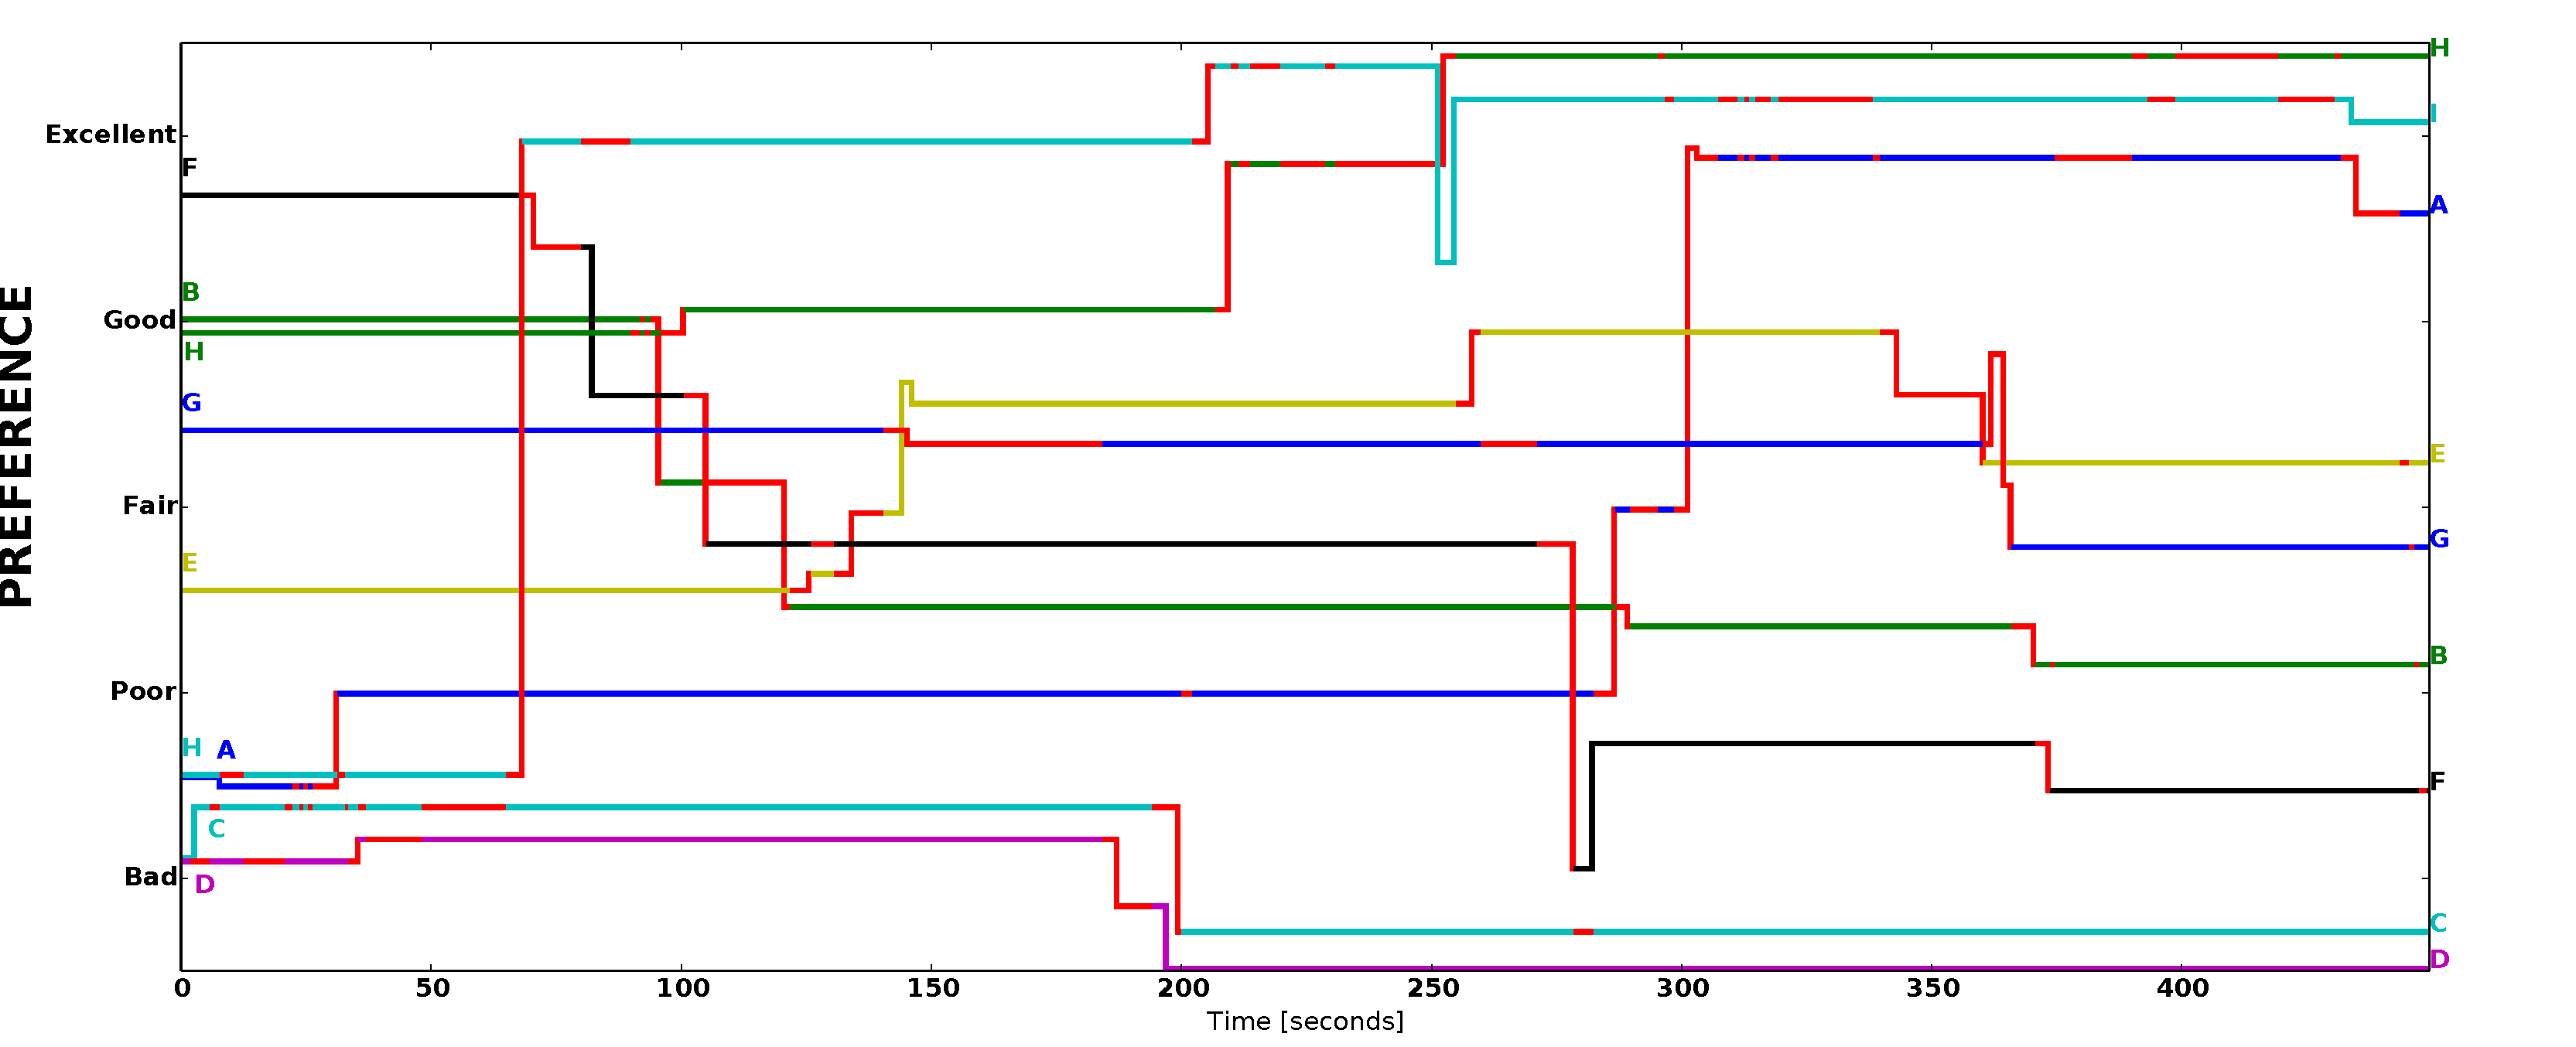
\includegraphics[width=.7\textwidth]{timeline.pdf}
	% 	\caption{This timeline of a single subject's listening test shows playback of fragments (red segments) and marker movements on the rating axis in function of time. }
	% 	\label{fig:timeline}
	% \end{figure*}
	For this reason, we include a proof-of-concept web page with:
	\begin{itemize}[noitemsep,nolistsep]
		\item All audioholder IDs, file names, subject IDs, audio element IDs, ... in the collected XMLs so far (\texttt{saves/*.xml})
		\item Selection of subjects and/or test samples to zoom in on a subset of the data %Check/uncheck each of the above for analysis (e.g. zoom in on a certain song, or exclude a subset of subjects)
		\item Embedded audio to hear corresponding test samples % (follow path in XML setup file, which is also embedded in the XML result file)
		\item Box plot, confidence plot, and scatter plot of rating values
		\item Timeline for a specific subject %(see Figure \ref{fig:timeline})%, perhaps re-playing the experiment in X times realtime. (If actual realtime, you could replay the audio...)
		\item Distribution plots of any radio button and number questions in pre- and post-test survey %(drop-down menu with `pretest', `posttest', ...; then drop-down menu with question `IDs' like `gender', `age', ...; make pie chart/histogram of these values over selected range of XMLs)
		\item All `comments' on a specific audioelement
		\item A `download' function for a CSV of ratings, survey responses and comments% various things (values, survey responses, comments) people might want to use for analysis, e.g. when XML scares them
		%\item Validation of setup XMLs (easily spot `errors', like duplicate IDs or URLs, missing/dangling tags, ...)
	\end{itemize}

\section{Concluding remarks and future work}
\label{sec:conclusion}
	
	The code and documentation can be pulled or downloaded from \url{code.soundsoftware.ac.uk/projects/webaudioevaluationtool}. 
	
	[Talking a little bit about what else might happen. Unless we really want to wrap this up. ]
	
	\cite{schoeffler2015mushra} gives a `checklist' for subjective evaluation of audio systems. The Web Audio Evaluation Toolbox meets most of its given requirements including remote testing, crossfading between audio streams, collecting browser information, utilising UI elements and working with various audio formats including uncompressed PCM or WAV format.
		% remote
		% language support (not explicitly stated)
		% crossfades
		% choosing speakers/sound device from within browser? --- NOT POSSIBLE, can only determine channel output counts and its up to the hardware to determine
		% collect information about software and sound system
		% buttons, scales, ... UI elements
		% must be able to load uncompressed PCM

	[What can we not do? `Method of adjustment', as in \cite{schoeffler2015mushra} is another can of worms, because, like, you could adjust lots of things (volume is just one of them, that could be done quite easily). Same for using input signals like the participant's voice. Either leave out, or mention this requires modification of the code we provide.]

%
% The following two commands are all you need in the
% initial runs of your .tex file to
% produce the bibliography for the citations in your paper.
\bibliographystyle{abbrv}
\bibliography{WAC2016}  % sigproc.bib is the name of the Bibliography in this case
% You must have a proper ".bib" file
%  and remember to run:
% latex bibtex latex latex
% to resolve all references
%
% ACM needs 'a single self-contained file'!
%
\end{document}
